\documentclass[12pt,a4paper]{scrreprt}
\usepackage[utf8]{inputenc}
\usepackage[english]{babel}
\usepackage{amsmath}
\usepackage{amsfonts}
\usepackage{amssymb}
\usepackage{pgfplots}
\usepackage{caption}
\usepackage{graphicx}
\usepackage{tikz-3dplot}
\usepackage{subcaption}
\usepackage{float}
\usepackage{adjustbox}
\usepackage{multirow,rotating}
\usepackage[autostyle]{csquotes}
\usepackage[toc,page]{appendix}

\usepackage[backend=biber,style=authoryear-comp]{biblatex}
\addbibresource{Meine Bibliothek.bib}

\begin{document}

\title{Market Definition of Platform Markets}
\date{\today}
\author{Ralf Dewenter, Ulrich Heimeshoff, Franziska Löw}

\maketitle

\chapter{Introduction}
The definition of the relevant market is a basic prerequisite for any political decision about possible market interventions. It is a competition policy concept with the aim to identify the competitive environment within an industry (\cite{argentesi_market_2005}). In case of a wrong understanding of the relevant market, regulatory interference might worsen the market situation, if for instance an antitrust authority imposes a socially inefficient regulation on an incumbent that in fact faces sufficient competition or blocks a welfare-enhancing merger. The objective of market definition is to search for the smallest set of products competing between them in order to guide the antitrust investigation. It therefore analyzes substitutional relationships between products or product groups to identify competitive constraints faced by a firm or a group of firms. If consumers can easily switch between two products, a firm will be constrained regarding the ability to raise prices (\cite{filistrucchi_market_2013}).

The reasoning of demand substitution is implemented in the conceptual tool of the so-called SSNIP (Small but Significant Non-transitory Increase in Price) test. According to this test, the narrowest market is defined as a set of products for which a hypothetical monopolist could sustainably raise prices above the current level by a given amount (usually 5\%-10\%) without losing demand. Following the European Commission "[…] differences in product characteristics are not in themselves sufficient to exclude demand substitutability […]” (\cite{european_commission_commission_1997}), which makes it necessary to define a market applying analytical tools like the SSNIP test. However, as we will explain below, in the context of two-sided markets this test needs further adaptations.

Two-sided markets, or platform markets, are characterized by intermediaries or platforms that sell two different products to two different groups of agents.\footnote{Two-sided markets are a special case of multi-sided markets, or platform markets. For simplicity, we will refer to two-sided markets, even though most of our argumentation is true for multi-sided markets.} These two groups are interconnected as they mutually influence each other’s demand. The platforms recognize the interconnection and choose the price structure according to the relative size of the indirect network effects. In a more restrictive definition of two-sided markets, \cite{rochet_platform_2003} determine those markets as two-sided, if the price structure is non-neutral, i.e., the volume of transactions and the participation levels vary as the price structure varies, holding the price level constant. This definition stresses the importance of the distinction between the price level, which is the sum of the prices charged by a platform on both sides, and price structure, which is the allocation of the price level among the two sides. Traditional antitrust instruments like the SSNIP test are designed for single-sided markets, using the price level to analyze a market. Drawing from the economic literature on market definition with interdependencies in demand, it can be shown that these instruments cannot easily be applied in case of two-sided platform competition (\cite{noel_analyzing_2005} \cite{filistrucchi_market_2013}).

Although two-sided markets are not invented by the digital revolution, digital markets very often demonstrate a market structure with two or more consumer-groups that are related via indirect network effects and are connected by platforms. A very prominent example can be found within the search engine market, where Google connects at least two market-sides: the demand for search query and the demand for placing advertisement. It can easily be seen, that advertisers value a big group on the other market side, as their scope and therefore the effectiveness of advertisement grows. The value of the search query on the other market side might be influenced negatively or positively by the amount of advertisement. This indirect network effect pretty much depends on the quality of the advertisement and on the consumers demand on personalized advertisement.

Two-sided markets can also be found within more traditional markets like credit cards, newspapers or shopping malls. These markets play an important role when analyzing the nature of two-sided markets as they offer an explicit market structure and available data. Requirements that cannot easily be found within digital markets due to rapidly changing market dynamics. Nevertheless, the rapid growth of digital markets calls for an analytical tool that can be applied to define the relevant market.

Based on economic reasoning we will explain why the application of a SSNIP test - being the most important analytical tool for regulatory and antitrust cases in the EU - on a two-sided market leads to a erroneous market definition. Furthermore we present an approach to analyze market structure by looking at the cross correlations of quantities of potential competitors. As a benchmark for the cross correlation coefficients we will simulate a Cournot duopol model. 

The paper proceeds as follows: chapter \ref{litrev} presents a review of the relevant literature on market definition and two-sided markets and analyses the consequences of applying a SSNIP test for market definition on two-sided markets; chapter \ref{model} presents a Cournot duopol model of platform competition and the results of a Monte Carlo simulation for this model; chapter \ref{empirical}  explains how we use empirical data to test our approach of market definition using cross-correlation functions of quantities in media markets.  


\chapter{Literature Review}\label{litrev}
This paper is related to a relatively recent line of economic literature, investigating the implications of two-sided markets on competition policy and offering different approaches to deal with the feedback effects between demand on multiple market sides. While the first policy contributions mainly criticized the application of standard policy to those markets (\cite{wright_one-sided_2004}; \cite{leonello_horizontal_2010}; \cite{chandra_mergers_2009}), more recent work has also intended to suggest alternative approaches (\cite{argentesi_estimating_2007}; \cite{song_estimating_2015}). We try to contribute to the latter by offering a new approach to define a two-sided market. 

The literature of two-sided markets was pioneered by the theoretical work of \cite{caillaud_chicken_2003}, \cite{rochet_platform_2003}, \cite{evans_antitrust_2003} and \cite{armstrong_competition_2006}, whereby the definition given by \cite{evans_antitrust_2003} can be seen as a particular case of the more general definition proposed by \cite{rochet_platform_2003} (\cite{filistrucchi_identifying_2012}). \cite{rochet_platform_2003} as well as \cite{armstrong_competition_2006} both provide a theoretical concept to analyze how platforms chose prices in a market with two consumer sides (networks) showing indirect network effects. However, there are a number of modeling differences between the two articles with regard to (a) the platform's cost structure, (b) the fee the consumers on both market sides have to pay and (c) the source of consumer heterogeneity. A more detailed discussion of these assumptions with regard to our approach is provided in Chapter \ref{model}.  

As mentioned above, earlier policy contributions criticize the application of standard competition policy on markets that exhibit at least one indirect network effect. \cite{evans_antitrust_2003}, \cite{evans_industrial_2007} \cite{wright_one-sided_2004} and \cite{kaiser_price_2006} are prominent examples of papers that have focused on competition policy on two-sided markets. They have pointed out, that in the presence of indirect network externalities the efficient price structure does not reflect the ratio of marginal cost, nor does increased competition necessarily leads to a more efficient market outcome or merger leads to increased prices.\footnote{\cite{malam_mergers_2011} uses an oligopoly model of competition with differentiated products (based on the approach of \cite{salop_monopolistic_1979}) where ad-sponsored media platforms charge a zero price to viewers when competing simultaneously for advertisers. He shows, that mergers among ad-sponsored platforms have a competition-intensifying effect, which offsets the incentive to increase prices on the advertiser side.} They show that relying on conventional methods to analyze mergers in two-sided markets will lead to significantly different results than using methods that explicitly incorporate the two-sided nature of those markets. \cite{evans_antitrust_2003} argues that defining a relevant market for antitrust purposes looking at only one side can lead to a market definition which is too narrow. In a more recent study \cite{evans_analysis_2008} analyze the Google and DoubleClick case, confirming, that the Lerner pricing formula does not hold for two-sided markets. While predatory pricing is a practice that harms competition in case of traditional industries\footnote{Industries with only one market side.}, selling a product below marginal cost\footnote{Or even for free, as is the case for the search-engine market as well as many digital markets.} can be a profit maximizing strategy rather than an attempt to predate in a two-sided market (\cite{wright_one-sided_2004}). \cite{wright_one-sided_2004} also argues, that increased competition does not necessarily lead to more efficient prices from the social point of view. An analysis of the Canadian newspaper industry shows, that mergers in two-sided markets may not necessarily lead to higher prices for either side of the market. Even a merger to monopoly might raise welfare and do so even in the absence of efficiency gains (\cite{leonello_horizontal_2010}). These papers emphasizes the need for alternative approaches to adopt competition policy that adequately hits the requirements of two-sided markets. 

The actual handling of antitrust issues regarding two-sided markets often lack the identification of indirect network effects. Even if indirect network effects are detected, the definition of the relevant market still remains a challenging task. This is mainly attributable to the fact that available analytical tools of market definition are not applicable for markets with interconnected demands as they consider price levels instead of price structure. The analysis of substitutional relationships is a well-established practice to define the relevant market. The European Commission uses the hypothetical monopolist test (the SSNIP test) which identifies the smallest relevant market through demand-substitutability of a certain product. If a small but significant, non-transitory price increase (5\% - 10\%) is profitable for the hypothetical monopolist then there is a relevant market (\cite{motta_competition_2004}). 

Using this analytical tools to define markets for a product offered on one side of a two-sided market can result in significantly overstating or understating the breadth of the market (\cite{evans_analysis_2008}). Due to the fact that platforms need to balance the preferences of two (or more) different groups of consumers, they often behave in a way that would not be efficient for traditional firms (e.g. they set prices $<$ marginal cost) (\cite{chandra_mergers_2009}).

\cite{evans_market_2012} uses the following example to illustrate the problem of the SSNIP test in platform markets. Suppose a small but significant, non-transitory price increase is profitable on one side under the assumption that nothing changes on the other market side of the platform included in the hypothetical monopoly. Therefore one could conclude that the products considered constitute a relevant antitrust market. However, a price increase on one side results in a reduction of demand by customers for that side and, through positive feedback effects, a reduction in the demand for the other side; the decline in demand on the other side further reduces the demand on the first side. Consequently, one might conclude after considering the positive feedback effects that the price increase is unprofitable. In that case the market is defined too narrowly .

The existence of positive feedback effects between demands of the two market sides calls for an optimal strategic behavior that varies widely from profit maximization on conventional one-sided markets. The SSNIP test might be applied in a modified way as shown by \cite{filistrucchi_market_2013} as well as \cite{evans_defining_2007}, who include the profit change in consideration of demand elasticity and indirect network effects. \cite{white_insulated_2012} present a UPP formulae for two-sided markets assuming that firms charge insulating tariffs, meaning that platforms choose quantities and then support those quantities by the corresponding insulating tariffs and \cite{noel_analyzing_2005} suggests an extension of the Critical Loss Analysis as an alternative method to define two-sided markets.\footnote{See \cite{evans_two-sided_2012} and \cite{filistrucchi_identifying_2012} for a discussion of market definition in two-sided markets.} Although these models are correct in theory, they show various problems when implemented in practice. 

\cite{filistrucchi_ssnip_2008} suggest a distinction of the two-sided markets regarding the observability of transaction costs.\footnote{Whereas \cite{filistrucchi_ssnip_2008} uses the terms “media type” and “payment card type”, \cite{filistrucchi_market_2013} use the terms “non-transaction” and “transaction” marktes.} In the "payment card type" market the platform can observe the transaction cost between the two market sides, whereas in the "media type" market the transaction cost does not exist (or is not observable to the platform, e.g. reader reads an ad). In \cite{filistrucchi_market_2013} the authors point out, that in two-sided non transaction markets, two (interrelated) markets need to be defined, while in transaction markets, only one market side should be defined. \cite{emch_market_2006} and \cite{alexandrov_antitrust_2011} show how a SSNIP test should be performed in a two-sided non transaction market. However, as transaction markets might exhibit asymmetric relationships in exceptional cases, this distinction cannot easily be applied. 

One well-known problem of most of those analytical tools is the procurement of necessary information. Due to the complexity of the two-sided market, this task is particularly difficult, as the scope of the indirect network effects has to be known for this analysis. A SSNIP test requires both qualitative data on substitutional behavior of consumers and quantitative market data. The data collection always is challenging, costly and time expensive and this is all the more true in case of two-sided markets as data has to be collected for two market sides. Even though the data required is available, two-sided markets poses special analytical challenges not allowing reliable conclusions about the market size. 

A determining factor are the platforms' pricing strategies. As mentioned above, price strategies have to be distinguished between the price level - the sum of the prices on both market sides - and price structure - the allocation of the price level among the two sides depending on the indirect network effects (\cite{rochet_two-sided_2006}). In an extreme case, prices on one market side can not be observed, as one market side benefits from a strong positive indirect network effect, affecting the other market side. In this case, the consumer group that receives the strong positive indirect network effect has to pay for the value gain. One market side therefore subsidizes the other depending on the relation of network effects. One can argue, that one market side does not pay a monetary price, but consumers pay with their attention or their data. The absence of monetary prices is not a rare phenomenon in digital markets. In the prominent example of the search engine market, the search market is subsidized by the advertiser market, because the extra value the advertiser side gets from an additional searcher is much higher, than the indirect network effect from the advertiser to the searcher\footnote{Which also can be assumed to be negative.}. Without monetary prices it will be impossible to analyze a hypothetical percentage price increase. To assign a value to the hedonic price, a quality benchmark is needed which itself is a difficult task (\cite{filistrucchi_market_2013}). Furthermore the consideration of prices does not capture the dynamic nature of a two-sided market, where firms rather use innovation and quality as strategic parameters (\cite{evans_economic_2002}; \cite{gual_market_2003}). 

The presence of relatively high fix cost and low marginal cost is another reason why the evaluation of prices does not represent an adequate measure, especially for online markets. In case of declining average cost due to fixed cost degression, the conventional SSNIP-test would define the relevant market to narrowly (\cite{gual_market_2003}). The same is true for endogenous sunk cost. In both cases  the relevant strategic parameters are others than the prices.

Beside the problems that arise when the SSNIP test is applied for two-sided markets, there are several general difficulties with this tool. The so called Cellophane-Fallacy  presents one well-known problem of the SSNIP-test (\cite{schaerr_cellophane_1985}). If the observed market price already exceeds the competitive price level, substitutional relationships between products are overestimated and market definition will be too broad. This problem is even more true for two-sided markets where a price on one market side seems to be “too low” (price is lower than monopoly price without feedback effects) while it is “too high” on the other market side (price is higher than monopoly price) (\cite{dewenter_einfuehrung_2014}).

A modified SSNIP test has to take into account all of these particular challenges when defining a two-sided market. Additional to this demanding task, the dynamic development of digital platform markets requires a fast and effective tool. The problems described make it evident that the SSNIP test – even in a modified way – is not an adequate tool when it comes to the task to define a relevant market that shows indirect network effects between two market sides, especially in the case of digital markets. This also applies for other analytical tools that analyze cross-price-elasticities. The reason is that market prices in two-sided markets cannot be interpreted in the conventional way as they reflect the relation of indirect network effects between the market sides. However, quantity measures offer an alternative approach to analyze substitutability of relevant goods. 

This paper contributes to the body of research that provides practical suggestions to practitioners. We use data on quantity to analyze substitutional effects on two-sided markets. The advantage of using quantity data is clear: As price levels and price structure in two sided markets are closely linked to the scope of indirect network effects, they can hardly be analyzed in the conventional way of antitrust economics. 

\chapter{A model of two-sided markets}\label{model}
In order to observe quantities from two-sided markets, we first develop a model of duopolistic platforms offering differentiated products (or services) to two different groups of users. Both sides of the market are assumed to be interrelated by indirect network effects and platforms to set quantities simultaneously. Consider therefore an industry with a continuum of potential users on each side $k = a,b$ of the market, with mass normalized to unity, and two platforms, $i = 1,2$, which enable the two groups to interact. Following \cite{shubik_market_1980} we introduce a quadratic utility function for each side of the market as\footnote{See also \cite{dixit_model_1979} and \cite{kind_competition_2006}}

\begin{equation}\label{4.1}
u_i^a = \nu^a q_i + \nu^a q_j-\frac{\beta^a q^2_i+ \beta^a q^2_j+ 2 \theta q_i q_j}{2}-(p_i-d s_i)q_i
\end{equation} and 

\begin{equation}\label{4.2}
u_i^b = \nu^b s_i + \nu^b s_j -\frac{\beta^b s^2_i+ \beta^b s^2_j+2 \mu s_i s_j}{2}-(r_i-g q_i)s_i.
\end{equation}

For $i=1,2, i \neq j$, we assume (i) $\nu^k > 0$, (ii) $\beta^k > 0$, (iii) $\beta^k>\vert\theta,\mu\vert$, where $\nu^k$ is a fixed benefit the agent obtains if she uses platform $i$ on market side $a$ or $b$ respectively.\footnote{\cite{weyl_price_2010} refers to it as the membership benefit or cost.} Parameter $\theta \in (0,1)$ and $\mu \in (0,1)$ indicate the degree of substitutability of both products, with $\theta (\mu) = 1$ indicating perfect substitutes and $\theta (\mu) = 0$ indicating monopolistic markets. $q_i$ and $s_i$ measure consumption of both product on platform $i$. By normalizing  population to one, we can interpret $q_i$ ($s_i$) as each individual’s consumption of product $i$ on market side $a$ ($b$), or as the network size of the platform $i$ on the respective market side.

The standard quadratic utility functions are also expanded by the cost-terms $(p_i-d s_i)q_i$ and $(r_i-g q_i)s_i$, respectively (\cite{kind_business_2009}). User's utility therefore depends on respective prices ($p_i$ and $r_i$) as well as on the network size of the opposite market side ($d$ and $g$). Hence, $d$ and $g$ describe the magnitude and the direction of the two indirect network effects. 

Solving for the FOCs of the consumer problem, given by $\frac{\delta u_i^a(q_i,q_j,s_i,p_i)}{\delta q_i}=0$ and  $\frac{\delta u_i^b(s_i,s_j,q_i,r_i)}{\delta s_i}=0$ utility can be expressed as

\begin{equation}\label{utility_a}
u_i^a = \nu^a-\beta^a q_i - \theta q_j +ds_i - p_i
\end{equation}
and
\begin{equation}\label{utility_b}
u_i^b=\nu^b-\beta^b s_i - \mu s_j +gq_i - r_i.
\end{equation} 

User heterogeneity on each side of the market can be modeled in two dimensions: the value of membership and the value of indirect network effects.\footnote{\cite{weyl_price_2010}, \cite{rochet_platform_2003} and \cite{armstrong_competition_2006} refer to this as the interaction value or the per-transaction value.} \cite{rochet_platform_2003} assume $v^k=0$ and that users have heterogeneous interaction values. Put differently, \cite{rochet_platform_2003} assume that the strength of indirect network effects vary with agents and platforms. \cite{armstrong_competition_2006}, in contrast, assumes that the indirect network effects $d,g$ only depend on the market side and allows for heterogeneous membership values.\footnote{\cite{rochet_platform_2003} as well as \cite{weyl_price_2010} allow agents to be heterogeneous along the two dimensions for the monopoly case.} We follow \cite{armstrong_competition_2006} in assuming that the scope of the indirect network effect depends on the market side, but not on agents or platforms. Our formulation of utility also coincides with \cite{armstrong_competition_2006} in that we assume lump-sum fees rather than per-transaction fees. 

Equations \ref{utility_a} and \ref{utility_b} can then be converted to obtain the inverse demand functions

\begin{equation}
p_i=\nu^a-\beta^a q_i - \theta q_j +ds_i
\end{equation}
and
\begin{equation}
r_i=\nu^b-\beta^b s_i - \mu s_j +gq_i.
\end{equation} 

This system of inverse demands illustrates the importance of assumption (iii): The closer $\theta, \mu$ to $\beta^k$, the closer substitutes are the two products, with $\theta, \mu \to \beta^ k$ as the limiting case. Equations \ref{4.1} and \ref{4.2} imply, that consumers utility from the indirect network effect is higher the more she uses the platform (\cite{kind_business_2009}). Keeping everything else equal, demand on market side $b$ has a positive impact on demand on market side $a$ if the indirect network parameter has a positive sign ($d > 0$). Same is true for market side $b$ and the parameter $g$. While most two-sided markets are characterized by two positive indirect network effects, especially ad-supported platforms such as media platforms are likely to show a positive as well as a negative effect. Demand for advertising increases with the size of media platform's audience. At the same time, when advertising is a nuisance to the audience, a higher amount of advertising would result in a lower demand for content.

Following \cite{armstrong_competition_2006}, we assume that the cost of platform $i$ is market-side specific and that they are incurred when an user joins the platform, so that platform's $i$ total cost is $c_i q_i+f_i s_i$ for some per-user cost $c_i$ for serving group $a$ and per-user cost $f_i$ for serving group $b$. The profit of platform $i$ therefore can be expressed as 

\begin{equation}\label{eq:profit}
\pi_i=(p_i-c_i)q_i+(r_i-f_i)s_i.
\end{equation}

Both platforms set $q_i$ and $s_i$ to maximize profits, given the choices of its rival. Substituting unique demands into \ref{eq:profit} for $i=1,2$, and using first order conditions, optimal quantities, prices and profits can be derived \footnote{See Appendix \ref{appendix_model} for optimal quantities}. Subsequently, optimal quantities can be used for simulating times series and correlation coefficients. 


 As optimal quantities are far from being easy to interpret, we present a simpler version of $q_i, s_i$ assuming $\nu^k, \beta^k=1$  as well as $c_i=f_i=0$. Equilibrium quantities are then

\begin{equation}\label{eq_quantities1}
	q_i=\frac{2+d+g+\mu}{4-(d+g)^2+\mu\theta+2(\mu+\theta)}
\end{equation}

and

\begin{equation}\label{eq_quantities2}
	s_i=\frac{2+d+g+\theta}{4-(d+g)^2+\mu\theta+2(\mu+\theta)}.
\end{equation}

As long as indirect network effects are positive, both quantities increase with $d$ and $g$. It can also be shown that $\frac{\partial q_i}{\partial \mu}<0$, $\frac{\partial q_i}{\partial (d+g)}>0$, $\frac{\partial s_i}{\partial \theta}<0$, $\frac{\partial s_i}{\partial (d+g)}>0$ as long as $0<(d+g)<2$. As positive indirect network effects have a positive impact on willingness to pay, quantities are also increasing with higher network effects. A higher degree of substitutability increases competition and reduces quantities.  

% --> Hab ich geändert und die partielle abl. von (d+g) aufgenommen. Sollen wir den Rechenweg in Anhang packen? 

\chapter{Monte Carlo Simulation}

We are interested in the market behavior of platforms depending on a change in parameters $d, g$ and $\theta, \mu$. More precisely our aim is to analyze the correlation coefficient of quantities depending on the degree of substitution and the indirect network effects. For this purpose, we use Monte Carlo simulation to obtain benchmark correlation coefficients, by simulating external shocks in platforms' marginal costs. 

We assume marginal costs to consist of two parts: (1) A market-specific term, which is common for both platforms and (2) an individual firm-specific cost-shock, assumed to occur in every period such that marginal costs follow a random walk (\cite[241]{harrington_detecting_2008}, \cite{paha_empirical_2011}). Assumption (1) is rational if we assume homogeneous input-factors are purchased from a perfectly competitive market. This assumption is relaxed by the platform-specific cost-shock which arises asymmetry between the platforms. This asymmetry might be due to individual negotiations between a platform and its service-provider. Moreover, asymmetry can be assumed to be larger, the smaller $\theta$ and $\mu$ as a high degree of heterogeneity might cause more asymmetric input costs, while homogeneous products should be produced with more symmetric input costs. 

% sind das wirklich n Märkte die wir simulieren? Oder n Zeitpunkte? Es sind keine voneinander abhängigen Zeitpunkte, deshalb märkte?

A cost function of platform $i$ for $n$ simulated markets with the corresponding characteristics can then be described as
\begin{equation}
f_{i,n} = a^a_n+a^a_{i,n},
\end{equation} and 
\begin{equation}
c_{i,n} = a^b_n+a^b_{i,n},
\end{equation}
with $a_{k,t} \in [0.001;0.0001]$ for the common cost shock and $a_{ki,t} \in [0.01;0.001] $ for the platform-specific cost shock. Cost-asymmetry among firms is therefore modeled by adding a firm-specific term $a_{ki,t}$ to the market-specific marginal cost. 

We randomly generate a dataset of $n=1000$ two-sided markets, by randomly generating $n=1000$ values for $f_i$ and $c_i$, respectively.\footnote{More precisely, we generate $n$ values for $a^a_n$ and $a^a_{i,n}$ and $a^b_n$ $a^b_{i,n}$ respectively.} Using the simulated values for $f_i$ and $c_i$ we are able to calculate the equilibrium quantities for every market on both market sides. As we are interested in substitutional relationship between the equilibrium quantities to define the market, we then calculate correlation coefficients from quantities. According to a Cournot duopoly we expect $q_i$ and $q_j$, as well as $s_i$ and $s_j$ to be correlated negatively. 

Figure \ref{fig_QQ} shows the relation between the sum of the indirect network effects $d+g$ and the correlation of quantities $\rho(q_i,q_j)$ on market side $a$, depending on the substitution parameter $\theta$ \footnote{for simplicity we assume $\mu=\theta$}. Keeping ($d+g$) constant, a high degree of homogeneity causes negative correlations to increase, which is consistent with what we would observe in markets without indirect network effects. Homogeneous products ($\mu=1$) cause a high degree of competition, which leads to high negative correlation of quantities, whereas a small degree of homogeneity $\theta \to 0$ show little or no substitutional effects. Keeping instead the correlation coefficient constant, an increasing total sum of indirect network effects suggests less competition. The higher the absolute amount of ($d+g$), the higher the negative correlation between the quantities keeping $\theta$ constant. As we assume network effects to be equal for both platforms, a higher interdependency of the markets will result in a higher correlation of quantities. 

Both, indirect network effects and parameters of product differentiation are unknown in our model. Therefore, in order to get a relative exact impression of substitutability, the strength of indirect network effects have to determined in advance. This can be achieved by either making theoretical assumptions about indirect network effects or by estimating these effects empirically. Most of the literature related to the quantification of the indirect network effects have based their analysis on electronic payments system industries (\cite{ackerberg_quantifying_2006}; \cite{rysman_empirical_2007}) or magazine and newspaper industries (\cite{kaiser_price_2006}, \cite{argentesi_estimating_2007}). Even though such an investigation on the INE gives empirical evidence, the drawback is twofold: First, many antitrust cases cannot meet the huge data requirements for an empirical investigation. Second, theoretical assumption have to be made that might not reflect the industry characteristics adequately. 

To overcome problems connected with data requirements and empirical modeling, we restrict our analysis to the assumptions of our theoretical model. By simulating quantities as a function of indirect network effects as well as differentiation parameters, we are able to estimate a range of substitutability depending on different strengths of the indirect network effects. Assuming a specific range of network effects and estimating correlation coefficients can then be used to limit the most likely range of substitutability.  


% Wir können ja nur eines aus dem anderen bestimmen, nicht beides gleichzeitig
% Das lassen wir daher erst einmal raus und schauen uns das später noch mal an. . 

\begin{figure}[H]
	\centering
	\caption{Simulated Correlation of $q_i$ and $q_j$}
	\begin{adjustbox}{width=\textwidth}	
	\input{QQ.tex}
	\label{fig_QQ}
\end{adjustbox}
\end{figure}

\chapter{Some Empirical Evidence}\label{empirical}
\section{Analyzing substitutional relationships in two-sided markets}

To test our approach of identifying substitutional relationships we use data on German popular magazines which are a typical example of two-sided markets. Magazine publishers serve a reader market as well as an advertising market, which are both interrelated by indirect network effects. Furthermore, data on German popular magazines is available for a broad range of products, for both, reader advertising markets. We are therefore able to identify possible substitutional products from a relatively high number of genres. Identification of possible substitutes has to be based on plausibility considerations. As popular magazines are typically highly differentiated, characteristics such as price level, layout, frequency of publication, but also socio-demographic factors of readers can help to identify possible competitors.  

As data form identical markets are typically affected by the same external influences, time series of prices and quantities are usually overlapped by common patterns. While quantities are strategic substitutes we expect to find negative contemporary correlations between substitutes. However, quantities as well as prices set by platforms from the same market or industry typically show identical patterns such as, e.g, seasonality, common trends or cyclical behavior. In order to prevent spurious regressions identical patterns have to be removed before an analysis of substitutability can be applied. For this purpose, we first apply different prewithening procedures. To prewhiten the quantities from both market sides we use different methods. At first, we apply a methods proposed by Dewenter (2003). All series from similar markets which show the same patterns are regressed on each other including a trend and a constant. Next, different time series models such as ARMA and ARIMA models are applied for prewhitening matters (see \cite{box_time_2008}). The results form different models are used for a comparison.

Next, we are able to calculate either simple correlation coefficients or cross correlation functions and to compare the results with simulated correlations. Using cross correlation functions instead of simple correlation coefficients allows us to analyze not only contemporary correlation but also possible effects such as shifts in quantities from one magazine to an other. These shifts typically occur with market entry of new products. Given that all competitors compete for a longer period, contemporary correlation coefficients should be an adequate measure. 

Even though a direct causality is not a necessary condition for detecting a substitutional relationship, Granger-causality test can be helpful to verify the results from the cross-correlation functions (\cite{dewenter_essays_2004}). In case that quantities are found to Granger--cause quantities form other magazines, it should be obcious that this might be due to substitutional relations. We therefore apply Granger--causility tests as a second measure. 

\section{Data}\label{sec:data}

Data used in this study is extracted from the online magazine database ``PZ Online'' (Public Magazines Online) which provides (inter alia) information on circulation, advertising volumes and prices for al high number of magazines form different genres.\footnote{PZ Online is provided by the German association of magazine publishers (Verband Deutscher Zeitschriftenverleger) to provide advertising customers with necessary information on possible advertising platforms.} In order to address rather different genres and markets we use data on news magazines as well as on women's and TV magazines. 

To account for quantities in reader and advertising markets we use circulation numbers and advertising pages per copy, respectively. 
Even though the dataset contains data from 2003 to date we restrict our analysis to different two and three-year intervals (see Table \ref{tab:sample selection} for an overview of our samples). The reasoning behind subsampling is two-fold: First, as data availability often plays a crucial role for any economic policy analysis, using shorter periods allows us to prove that our approach is suitable even with low data availability. 
Second, antitrust concerns are often related to certain periods as markets develop constantly. Additionally, during recent years, print media have been subject to decreasing circulation and declining advertising revenues due to digitalization \footnote{For more information see \cite{cabyova_impact_2014} or \cite{picard_digitization_2011}}. Using data on magazine products proves that also markets with either decreasing or increasing market volumes can be subject of our approach.
\end{enumerate}

\begin{center}
\begin{table}[htbp]
	
	\caption{Subsamples}
\begin{adjustbox}{width=\textwidth}	
\begin{scriptsize}
\bigskip\begin{tabular}{llllllll}
\hline 
	 Segment 	& Titles & & & Period &  & Frequency & Obs \\ \hline
	 &  &  &  & Begin & End &  &  \\ \hline
	News magazines 		& FOCUS & Der Spiegel & Stern & 2004 / 33 & 2006 / 33 & weekly & 105 \\ \hline
										&  &  &  & 2013 / 33 & 2015 / 33 & weekly & 105 \\ \hline
	TV magazines 			& TV Movie & TV Spielfilm & TV Digital & 2012 / 15 & 2015 /15 & biweekly & 79 \\ \hline
	Women's magazines	& Brigitte & Freundin & Für Sie & 2012 / 15 & 2015 /15 & biweekly & 79 \\ \hline
\end{tabular}
\end{scriptsize}
	\label{tab:sample selection}
\end{adjustbox}
\end{table}
\end{center}

\subsection*{News Magazines} 

First published in 1947 ``Der Spiegel'' had a monopoly on investigative journalism for a long time when Burda-Verlag entered the market in 1993 with a news magazine, FOCUS, claiming itself to be a close substitute to Der Spiegel. The latter instead opposed that FOCUS is an illustrative magazine similar to Stern, a magazine first published in 1946 by Gruner + Jahr \cite{kaltenhaeuser_abstimmung_2005}. In fact all three magazines differ regarding their editorial concept. Der Spiegel mainly focuses on complex political and social issues, whereas FOCUS also covers more non-political topics such as health and fitness. Stern has been a simple illustrative magazine without any political appeal until the 60s. It then started to address current political topics (\cite{vogel_populaere_1998}). Even though all three magazines have different editorial concepts, readership of Der Spiegel, FOCUS and Stern does not differ significantly regarding their socio-demographic characteristics, but their political orientation: While FOCUS is rather a conservative outlet, the coverage of Der Spiegel can be considered as left-wing. Stern which reporting is less political, can be located somewhere in between (\cite{kaltenhaeuser_abstimmung_2005}). Having this in mind, we do not expect strong competition in the reader market between the magazines as, e.g., a "left-wing" reader of Der Spiegel would probably not consider FOCUS as an adequate substitute et vice versa.\footnote{However as some of the readers might not have strong political preferences, we expect some kind of contemporary negative correlation, as final purchasing decisions will be influenced by cover stories and content. This assumption is supported by the fact that subscription is just a minor part of total sales (about 2-3 $\%$). We assume, if any, weak negative indirect network effects from the advertising market as the share of advertising pages per copy ranges between 2$\%$ and 8$\%$.} All three magazines offer several digital services (website and mobile apps) with mostly free content. 

Advertising demand on the other side is assumed to be strongly affected by the size and the characteristics of the readership of a certain magazine. However, in contrast to the reader market, political orientation should not matter as much as socio-demographic characteristics. We therefore expect the the degree of substitutability to be higher in the advertising market. All of the magazines moght therefore be competitors in the advertising market.  

Graphical inspection of quantities (see figures ?? and ??) as well summary statistics (see tables \ref{appendix_sum_fss} and), show that in the reader market Stern and Der Spiegel have similar sales, whereas circulation of FOCUS is considerably smaller. However, quantities in the advertising market of all three magazines are quite similar and also show seasonal fluctuations. However, quantities in both markets have as expected declined for all products over time.  

\subsubsection{Reader Market}
Figure \ref{fig_ccf_circ_fss} shows relatively small cross-correlation coefficients on the reader market, indicating weak substitutional relationships between the magazines.\footnote{In the figure $t<0$ indicates the correlation between the current sales of the first magazine and the lagged sales of the second magazine. The dashed lines represent the standard error bounds.} Furthermore the coefficients show, that the relationship has changed over the two periods.\footnote{The corresponding values are listed in \ref{tab_CCF}} Even if all contemporary values are negative, indicating that the magazines are rather substitutes, not all are statistically significant. In the earlier period only the contemporary crosscorrelation coefficients of the pairs FOCUS and Der Spiegel (-0.25) and Der Spiegel and Stern (-0.23) are statistically significant, showing weak substitutional relationship. In the later sample, the contemporary substitutional effect between FOCUS and Der Spiegel disappeared (-0.07), whereas it intensified between Der Spiegel and Stern (-0.36). However, there is a positive significant intertemporal coefficient at the first lag for the pair FOCUS and Der Spiegel (-0.27). \\

\begin{figure}[H]\footnote{(1) = 2004w33-2006w33, (2) = 2013w33-2015w33}
\caption{CCF Reader Market (R.M.)}
\label{fig_ccf_circ_fss}
	\centering
	\includegraphics[scale=.6]{ccf_circ_fss.eps}
\end{figure}

The results of the Granger-causality test for the adjusted time series are listed in \ref{tab_granger_fss}. For the earlier sample the null hypothesis (sales of one magazine do not Granger-causes sales of the other two magazines) cannot be rejected at the usual level of confidence, except for the  influence of Stern on FOCUS and Der Spiegel. In the later sample Granger causality test suggests, that Der Spiegel Granger-causes Focus and Stern Granger-causes Focus and Der Spiegel. Interpreting both the correlation coefficients and the Granger causality test, substitutional relationships, if any, can be detected between Der Spiegel and Stern in both samples. 

\begin{table}[!htbp] \centering 
  \caption{Granger Causality test} 
  \label{tab_granger_fss} 
\begin{tabular}{@{\extracolsep{5pt}} lll} 
\\[-1.8ex]\hline 
\hline \\[-1.8ex] 
 & Test-statisitcs \\ 
\hline \\[-1.8ex] 
2004-2006 & Sales & Ad Pages/Copy\\
\hline \\[-1.8ex]
Focus --\textgreater  Der Spiegel & $.77536$ & $4.3234^{**}$\\ 
Focus --\textgreater  Stern & $.65988$ & $6.0462^{**}$ \\  
\hline
Der Spiegel --\textgreater  Focus & $.08055$ & $.95385$\\ 
Der Spiegel --\textgreater  Stern & $.26141$ & $1.1025$\\  
\hline
Stern --\textgreater  Focus & $9.9076^{***}$ & $8.411^{***}$  \\ 
Stern --\textgreater  Der Spiegel & $13.586^{***}$ & $9.1812^{***}$ \\ 
\hline \\[-1.8ex] 
2013-2015 \\
\hline \\[-1.8ex] 
Focus --\textgreater  Der Stern & $ .65092$ & $ 11.338^{***}$\\ 
Focus --\textgreater  Stern & $1.4738$ & $6.1756^{***}$ \\  
\hline
Der Spiegel --\textgreater  Focus & $6.2475^{**}$ & $.00104$ \\ 
Der Spiegel --\textgreater  Stern & $.02581$ & $ 1.3149^{*}$ \\ 
\hline
Stern --\textgreater  Focus & $3.6629^{*}$ & $ 6.8459^{**}$\\ 
Stern --\textgreater  Der Spiegel & $3.1919^{*}$ & $3.8729^{**}$\\ 
\hline \\[-1.8ex]
\end{tabular} 
\end{table}
 

\par\medskip

\subsubsection{Advertising Market}
Turning to the advertising market, figure \ref{fig_ccf_ads_fss} supports the assumption, that competition on this market side is stronger.\footnote{The corresponding values are listed in \ref{tab_ccf_ads_fss}.} In contrast to the reader market, all contemporary correlations are statistically significant and negative. In the first sample we can find substitutional relationship among all three magazines, with a contemporary negative correlation of $-0.65$ for FOCUS / Der Spiegel being the strongest. FOCUS and Stern show a rather weak substitutional relationship ($-0.31$), and a contemporary correlation for Stern and Der Spiegel of $-0.42$. In the second time period competition seems to have decreased between FOCUS and Der Spiegel, as the correlation coefficient is -0.31. Der Spiegel and Stern now show the strongest substitutional relationship (-0.44) and the weakest correlation is between FOCUS and Stern (-0.25). It is striking that some of the intertemporal effects of FOCUS and Der Spiegel are positive and significant. This phenomenon might be due to a common trend, that has not been filtered in the first stage. Because of the weekly data, a separated seasonal adjustment could only be carried out with an enormous effort, as irregular effects such as calendar effects or moving festivals appear within the time series (\cite{harvey_modeling_1997}). Such common structural trends are assumed to have a positive rather than a negative influence on the results. 


\begin{figure}[H]
\caption{CCF advertising pages/copy (A.M.)}
	\centering
	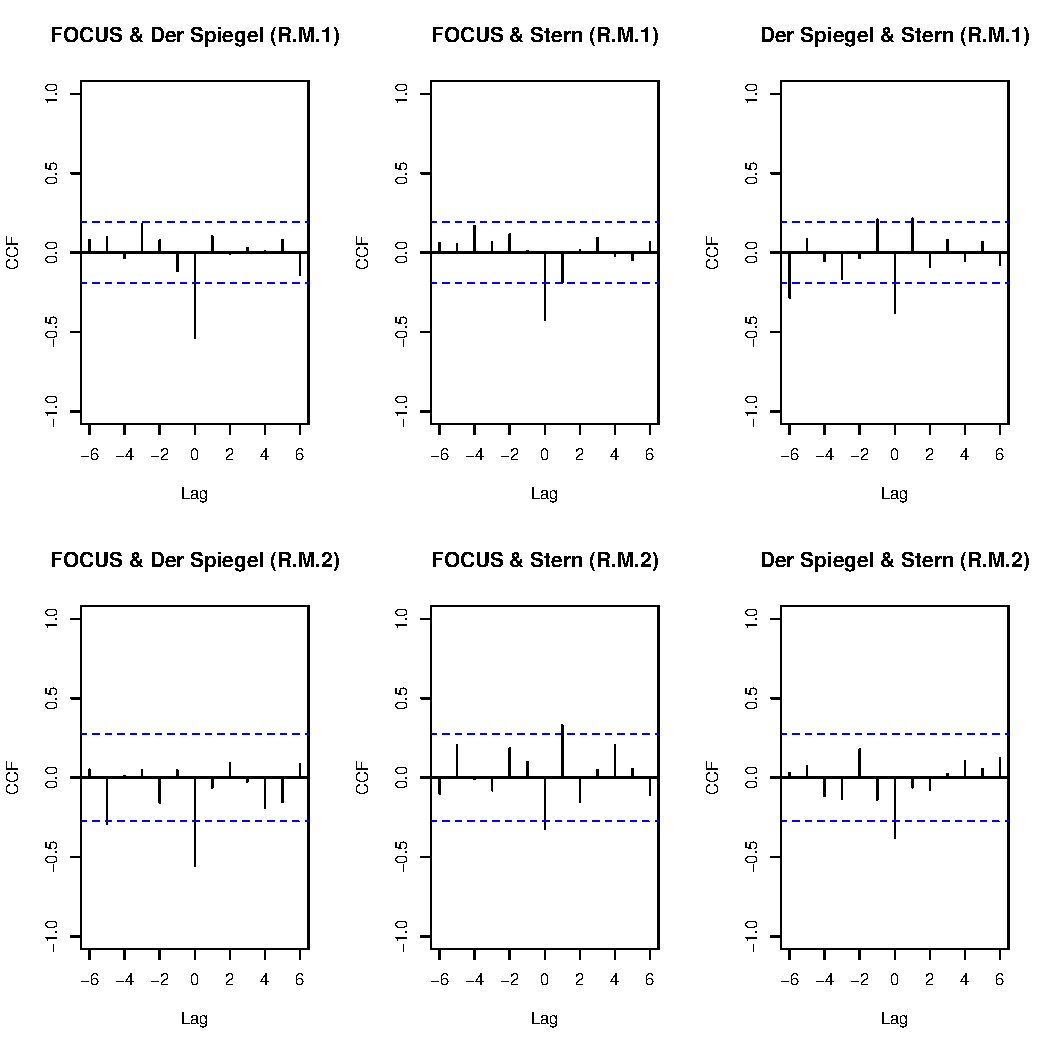
\includegraphics[scale=.5]{ccf_ads_fss.eps}
	\label{fig_ccf_ads_fss}
\end{figure}

The values of the Granger-causality test of adjusted time series mainly support the results of the correlation coefficients. Only the Granger-causality of Der Spiegel on the respective other two magazines (in the earlier sample) an on FOCUS (in the later sample) cannot be verified at a 10$\%$ significance level. 

\subsubsection{Comparison with Benchmark}
Comparing these coefficients with the benchmark model - assuming that total INE (from reader market to advertising market and reverse) exist and are positive -  the following conclusions can be drawn: On the reader market, contemporary correlation coefficients suggest, that FOCUS / Der Spiegel and Stern / Der Spiegel most closely resemble each other ($\theta\approx0.2-0.3$). In the later sample the substitutional relationship between Der Spiegel and Stern intensified ($\theta\approx0.3$). 
However, on the advertising market side, substitutional relationship between FOCUS / Der Spiegel is stronger than on the reader market side, as the degree of competition can assumed to range between $\theta=0.5$ and $\theta=0.7$ for the time period 2004-2006, depending the strength of the INE. The relationship between the INE and the corresponding degree of competition is shown in \ref{fig_QQ_fss}, where the upper line represents the contemporary correlation between sales of FOCUS / Der Spiegel in the reader market for the earlier sample and the lower line shows the estimated cross correlation on the advertising market: The higher the assumed sum of INE, the lower is the indicated $\theta$. To put it in another way, the same negative correlation coefficients indicate less competition if the INE is high. For instance, if we assume, that the sum of INE ranges between 0.1 and 0.4, we can find a degree of homogeneity of $\theta=0.7$ on the advertising market, whereas INE of 0.7 to 0.9, indicate $\theta=0.5$. In the later sample, negative correlation between FOCUS / Der Spiegel decreased (-0.31), suggesting a degree of homogeneity of $\theta\approx0.3$ (or $\theta\approx0.2$ if we assume $d+g>0.8$). A similar analysis can be made for the substitutional relationship of FOCUS / Stern and Der Spiegel / Stern. The contemporary correlation of both of the pairs has not greatly varied between both periods, indicating a degree of competition of $\theta\approx0.3$ for FOCUS / Stern and $\theta\approx0.5-0.4$. 

\begin{figure}[H]
	\centering
	\caption{Degree of competition FOCUS $\&$ Der Spiegel 2004-2006}
	\label{fig_QQ_fss}
	\begin{adjustbox}{width=\textwidth}	
	\input{QQ_fss.tex}
\end{adjustbox}
\end{figure}
  
 
\subsubsection{Conclusions}
This chapter carried out an empirical analysis of the market of german news magazines using cross-correlation functions to suitable determine substitutional, complementary and indifferent relations between FOCUS, Stern and Der Spiegel. As a first striking result, the substitutional relationship is stronger on the advertising market side for all combinations of the magazines. This result strongly supports the assumption of the dichotomy of the two market sides with respect to a market definition.  

Furthermore, the contemporary correlation on the advertising market decreased between the two periods for FOCUS / Der Spiegel, and slightly increased for FOCUS / Stern and Der Spiegel / Stern. However, the degree of competition between the last two pairs can be assumed to have remained the same. But still, the overall competition on the advertising market seems to have diminished, possibly caused by new, digital advertising possibilities constituting new substitutes for advertising demand. 

Turning to the reader market contemporary substitutional relationship also decreased between the periods regarding FOCUS / Der Spiegel, whereas Der Spiegel / Stern seem to became stronger substitutes. This might be due to a change in the editorial concept of one or both magazines. FOCUS and Stern did not show any significant substitutional relationship in both samples.  

Overall, the empirical results support the assumption, that the three magazines rather build a common market on the advertising market, but seem to claim own sub-markets on the reader market within both time samples. However, in the later sample, new advertising possibilities smoothen the competition on the advertising market. 

\subsection{Program Guides}
A similar analysis was conducted for the market of program guides, including the magazines TV-Movie, TV-Spielfilm and TV-Digital. Considering figure \ref{fig_tv} and the corresponding summary statistics, a common structural trend is detectable for the sales as well as for the advertising volumes of all three magazines. However, on both market sides the time series of TV Digital seems to differ from the remaining two program guides. The sales of TV-Movie and TV-Spielfilm are similar in levels, whereby the sales of TV-Digital are considerably higher. On the other market side, advertising volumes of all three magazines develop similar in the beginning of the time sample, but start to diverge in 2013 as advertising volumes of TV-Digital are slightly higher. Even though a negative correlation is not recognizable from the figures, the differences between TV-Digital and the other two magazines might be a first reference to different degrees of substitution among the variables. We expect that the degree of substitution between TV-Movie and TV-Spielfilm is the highest. And again, substitutional relationship on the advertising market is supposed to be stronger, as advertiser do not care much about personal preferences of the reader, but rather about sociodemographic qualities. On the other hand, reader might have a strong preference for one program guide, because they are used to the structure of the magazine. 
In figure \ref{fig_ccf_tv} the crosscorrelation functions of the reader market (R.M.) and the advertising market (A.M.) supports the assumptions. The magnitude of the contemporal correlation among TV-Movie and TV-Spielfilm is the strongest on both market sides: It is of -.44 on the reader market and -.56 on the advertising market. Comparing these results with our benchmark model, and assuming positive INE, the competition parameter ranges between $\theta=.3-.5$ on the reader market side and $\theta=.4-.6$ on the advertising market side. Again, the degree of competition depends on the sum of the indirect network effects: the higher the assumed INE, the lower the competition parameter for the same correlation coefficient. Contemporary correlation between TV-Movie and TV-Digital is significant but small: -.28 on the reader market and -.29 on the advertising market, indicating a degree of competition of $\theta\approx.3$ on both market sides. No significant correlation can be found between TV-Spielfilm and TV-Digital

\begin{figure}[H]
\caption{CCF program guides}
\label{fig_ccf_tv}
	\centering
	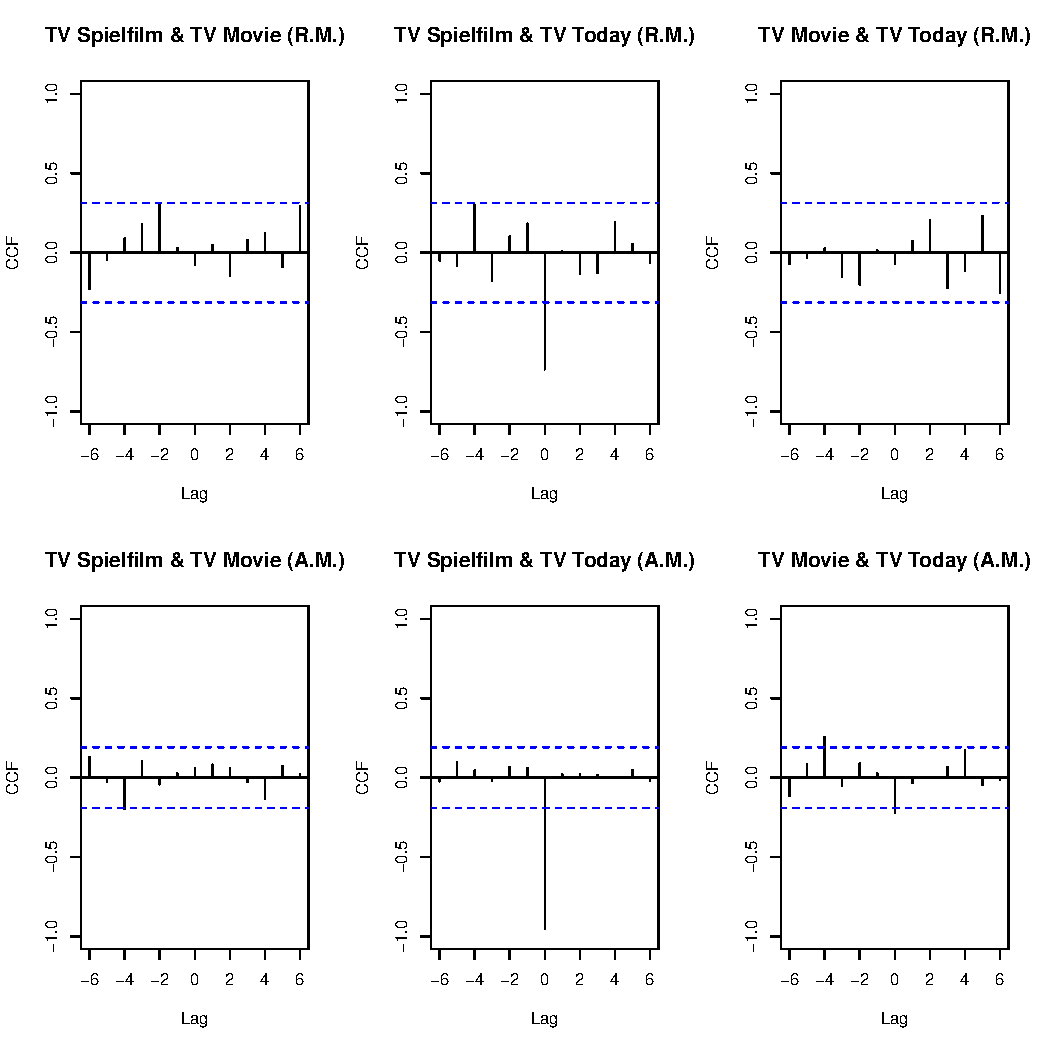
\includegraphics[scale=.6]{ccf_tv.eps}
\end{figure}


\subsection{Women's Magazines}
Turning to biweekly women's magazines, we analyzed sales and advertising volumes of the three magazines Brigitte, Freundin and Für Sie. As one can see in figure \ref{fig_frauen} sales of Brigitte are the highest, followed by Freundin and Für Sie. On the advertising market the number of advertising pages of Freundin is the highest, closely followed by Brigitte, whereas the number of advertising pages of Für Sie is smaller. Again, the quantities on both market sides do not show indications of negative correlations. However, as the time series seem to follow a common structural trend, the assumption of a substitutional relationship is reasonable. The ccf of the adjusted time series are shown in figure \ref{fig_ccf_frauen}. As a striking outcome, contemporal correlation on the reader market is rather small for all three cases. It is -.25 for both Brigitte / Freundin and Freundin / Für Sie, suggesting a degree of homogeneity of $\theta=.2-.3$. However, on the advertising market contemporal correlation between Brigitte and Freundin is relative large (-.7), whereas contemporal correlation of Brigitte / Für Sie (-.27) and Freundin / Für Sie (-.24) is smaller, but still significant. The high correlation of Brigitte and Freundin indicates a degree of competition of $\theta=.5-.8$, and for the other two magazine pairs we find $\theta=.2-.3$. 


\begin{figure}[H]
\caption{CCF women's magazines}
\label{fig_ccf_frauen}
	\centering
	\includegraphics[scale=.6]{ccf_frauen.eps}
\end{figure}

\begin{table}[!htbp] \centering
	\caption{Contemporary correlations}
	\label{tab_CCF}
\begin{tabular}{@{\extracolsep{5pt}} lll}
\\[-1.8ex]\hline 
\hline \\[-1.8ex]
	news magazines(1) & sales & ad pages/copy \\
	\hline
	FOCUS \& Der Spiegel & -.246 & -.633 \\
	FOCUS \& Stern & -.062 & -.306 \\
	Der Spiegel \& Stern & -.232 & -.445 \\
	\hline
	news magazines(2) & & \\
	\hline
	FOCUS \& Der Spiegel & -.072 & -.308 \\
	FOCUS \& Stern & -.043 & -.245 \\
	Der Spiegel \& Stern & -.364 & -.436 \\
	\hline
	program guides & & \  \\ 
	\hline
	TV-Movie \& TV-Spielfilm & -.443 & -.558 \\
	TV-Movie \& TV-Digital & -.281 & -.285 \\
	TV-Spielfilm \& TV-Digital & .077 & -.135 \\ 
	\hline
	women's magazines &  & \  \\ 
	\hline
	Brigtte \& Freundin & -.248 & -.697 \\ 
	Brigitte \& Für Sie & -.040 & -.267 \\ 
	Freundin \& Für Sie & -.252 & -.241 \\ \hline
\end{tabular}
	\end{table}

\subsection{program guides / Women's Magazines }

\begin{figure}[H]
\caption{CCF women's magazines / program guides}
\label{}
	\centering
	\includegraphics[scale=.5]{ccf_tvfrauen.eps}
\end{figure}



\begin{appendices}


\chapter{Model}

\subsection{Profit Maximization}\label{appendix_model}


\subsection{Monte Carlo Simulation}

\begin{table}[ht] \centering 
\caption{Simulated Correlation Coefficients of $q_1$ and $q_2$}
\label{tab_ccf_simulated}
\begin{adjustbox}{width=\textwidth}	
\small
\begin{tabular}{@{\extracolsep{5pt}} cccccccccccc} 
\\[-1.8ex]\hline 
\hline \\[-1.8ex] 
$d+g$ & $\theta=0$ & $\theta=.1$ & $\theta=.2$ & $\theta=.3$ & $\theta=.4$ & $\theta=.5$ & $\theta=.6$ & $\theta=.7$ & $\theta=.8$ & $\theta=.9$ & $\theta=1$\\ 
\hline \\[-1.8ex] 
-.9 & $0.010$ & $$-$0.178$ & $$-$0.321$ & $$-$0.477$ & $$-$0.616$ & $$-$0.722$ & $$-$0.824$ & $$-$0.885$ & $$-$0.941$ & $$-$0.974$ & $$-$0.994$ \\ 
-.8 & $0.025$ & $$-$0.152$ & $$-$0.264$ & $$-$0.423$ & $$-$0.558$ & $$-$0.644$ & $$-$0.775$ & $$-$0.839$ & $$-$0.907$ & $$-$0.946$ & $$-$0.979$ \\ 
-.7 & $$-$0.002$ & $$-$0.130$ & $$-$0.313$ & $$-$0.374$ & $$-$0.499$ & $$-$0.622$ & $$-$0.691$ & $$-$0.794$ & $$-$0.858$ & $$-$0.917$ & $$-$0.953$ \\ 
-.6 & $0.007$ & $$-$0.086$ & $$-$0.265$ & $$-$0.430$ & $$-$0.488$ & $$-$0.574$ & $$-$0.650$ & $$-$0.751$ & $$-$0.837$ & $$-$0.891$ & $$-$0.921$ \\ 
-.5 & $$-$0.019$ & $$-$0.098$ & $$-$0.197$ & $$-$0.289$ & $$-$0.437$ & $$-$0.572$ & $$-$0.605$ & $$-$0.712$ & $$-$0.786$ & $$-$0.855$ & $$-$0.897$ \\ 
-.4 & $$-$0.003$ & $$-$0.067$ & $$-$0.226$ & $$-$0.264$ & $$-$0.395$ & $$-$0.507$ & $$-$0.582$ & $$-$0.692$ & $$-$0.758$ & $$-$0.822$ & $$-$0.865$ \\ 
-.3 & $0.049$ & $$-$0.100$ & $$-$0.156$ & $$-$0.264$ & $$-$0.414$ & $$-$0.519$ & $$-$0.553$ & $$-$0.643$ & $$-$0.694$ & $$-$0.790$ & $$-$0.831$ \\ 
-.2 & $$-$0.021$ & $$-$0.117$ & $$-$0.207$ & $$-$0.324$ & $$-$0.345$ & $$-$0.462$ & $$-$0.576$ & $$-$0.627$ & $$-$0.691$ & $$-$0.767$ & $$-$0.816$ \\ 
-.1 & $0.035$ & $$-$0.095$ & $$-$0.192$ & $$-$0.321$ & $$-$0.363$ & $$-$0.420$ & $$-$0.569$ & $$-$0.626$ & $$-$0.713$ & $$-$0.745$ & $$-$0.800$ \\ 
0 & $0.014$ & $$-$0.099$ & $$-$0.221$ & $$-$0.312$ & $$-$0.444$ & $$-$0.501$ & $$-$0.556$ & $$-$0.595$ & $$-$0.669$ & $$-$0.774$ & $$-$0.792$ \\ 
.1 & $0.007$ & $$-$0.134$ & $$-$0.213$ & $$-$0.314$ & $$-$0.386$ & $$-$0.472$ & $$-$0.526$ & $$-$0.634$ & $$-$0.708$ & $$-$0.748$ & $$-$0.793$ \\ 
.2 & $0.031$ & $$-$0.093$ & $$-$0.194$ & $$-$0.253$ & $$-$0.419$ & $$-$0.521$ & $$-$0.555$ & $$-$0.666$ & $$-$0.693$ & $$-$0.796$ & $$-$0.818$ \\ 
.3 & $0.057$ & $$-$0.113$ & $$-$0.244$ & $$-$0.316$ & $$-$0.387$ & $$-$0.440$ & $$-$0.595$ & $$-$0.637$ & $$-$0.746$ & $$-$0.800$ & $$-$0.838$ \\ 
.4 & $0.070$ & $$-$0.111$ & $$-$0.197$ & $$-$0.312$ & $$-$0.407$ & $$-$0.541$ & $$-$0.592$ & $$-$0.673$ & $$-$0.759$ & $$-$0.823$ & $$-$0.859$ \\ 
.5 & $0.017$ & $$-$0.176$ & $$-$0.219$ & $$-$0.287$ & $$-$0.452$ & $$-$0.499$ & $$-$0.661$ & $$-$0.736$ & $$-$0.779$ & $$-$0.835$ & $$-$0.901$ \\ 
.6 & $0.010$ & $$-$0.070$ & $$-$0.266$ & $$-$0.384$ & $$-$0.496$ & $$-$0.580$ & $$-$0.641$ & $$-$0.753$ & $$-$0.824$ & $$-$0.885$ & $$-$0.923$ \\ 
.7 & $0.006$ & $$-$0.092$ & $$-$0.241$ & $$-$0.356$ & $$-$0.536$ & $$-$0.622$ & $$-$0.728$ & $$-$0.795$ & $$-$0.870$ & $$-$0.923$ & $$-$0.956$ \\ 
.8 & $$-$0.006$ & $$-$0.111$ & $$-$0.262$ & $$-$0.455$ & $$-$0.543$ & $$-$0.667$ & $$-$0.752$ & $$-$0.840$ & $$-$0.900$ & $$-$0.959$ & $$-$0.980$ \\ 
.9 & $0.008$ & $$-$0.143$ & $$-$0.304$ & $$-$0.463$ & $$-$0.612$ & $$-$0.731$ & $$-$0.815$ & $$-$0.891$ & $$-$0.935$ & $$-$0.976$ & $$-$0.994$ \\
\hline \\[-1.8ex] 
\end{tabular} 
\end{adjustbox}
\label{tab:ccf_sim}
\end{table} 


\chapter{Empirical Analysis}

\section{Summary Statistics}

\subsection{News Magazines}  \label{appendix_sum_fss} 

\begin{figure}[H]
\caption{Reader Market}
\begin{minipage}
	\centering
	\input{circ_fss1.tex}
\end{minipage}
\hfil
\begin{minipage}
	\centering
	\input{circ_fss2.tex}
\end{minipage}
\end{figure}

\begin{figure}[H]
\caption{Advertising Market}
\begin{minipage}
	\centering
	\input{ads_fss1.tex}
\end{minipage}
\hfil
\begin{minipage}
	\centering
	\input{ads_fss2.tex}
\end{minipage}
\end{figure}

\begin{table}[!htbp] \centering 
  \caption{Summary Statistics: sales of news magazines} 
\begin{tabular}{@{\extracolsep{5pt}}lccccc} 
\\[-1.8ex]\hline 
\hline \\[-1.8ex] 
Statistic & \multicolumn{1}{c}{N} & \multicolumn{1}{c}{Mean} & \multicolumn{1}{c}{St. Dev.} & \multicolumn{1}{c}{Min} & \multicolumn{1}{c}{Max} \\ 
\hline \\[-1.8ex] 
2004-2006 \\
\hline \\[-1.8ex] 
FOCUS & 105 & 170,251.6 & 34,249.7 & 111,395 & 275,025 \\ 
Der Spiegel & 105 & 442,253.9 & 49,154.8 & 334,815 & 548,854 \\ 
Stern & 105 & 395,619.7 & 41,844.5 & 306,323 & 499,818 \\ 
\hline \\[-1.8ex] 
2013-2015 \\
\hline \\[-1.8ex] 
FOCUS & 105 & 78,641.3 & 20,105.1 & 48,179.0 & 184,981.0 \\ 
Der Spiegel & 105 & 249,184.4 & 23,247.2 & 203,587 & 320,651 \\ 
Stern & 105 & 215,036.0 & 18,908.1 & 174,604 & 272,927 \\  
\hline \\[-1.8ex] 
\end{tabular} 
\end{table} 

\begin{table}[!htbp] \centering 
  \caption{Summary Statistics: advertising pages/copy of news magazines} 
\begin{tabular}{@{\extracolsep{5pt}}lccccc} 
\\[-1.8ex]\hline 
\hline \\[-1.8ex] 
Statistic & \multicolumn{1}{c}{N} & \multicolumn{1}{c}{Mean} & \multicolumn{1}{c}{St. Dev.} & \multicolumn{1}{c}{Min} & \multicolumn{1}{c}{Max} \\ 
\hline \\[-1.8ex] 
2004-2006 \\
\hline \\[-1.8ex] 
FOCUS & 105 & 35.597 & 5.768 & 18.140 & 45.698 \\ 
Der Spiegel & 105 & 33.367 & 7.980 & 13.201 & 48.438 \\ 
Stern & 105 & 35.335 & 5.224 & 21.744 & 42.268 \\ 
\hline \\[-1.8ex] 
2013-2015 \\
\hline \\[-1.8ex] 
FOCUS & 104 & 24.396 & 5.458 & 14.782 & 40.552 \\ 
Der Spiegel & 104 & 19.506 & 4.380 & 10.356 & 28.756 \\ 
Stern & 105 & 22.599 & 4.253 & 13.281 & 32.359 \\ 
\hline \\[-1.8ex] 
\end{tabular} 
\end{table} 

\subsection{Program Guides}\label{appendix_sum_tv}

\begin{figure}[H]
\caption{program guides}
	\label{fig_tv}
\begin{minipage}
	\centering
	\input{circ_tv.tex}
\end{minipage}
\hfil
\begin{minipage}
	\centering
	\input{ads_tv.tex}
\end{minipage}
\end{figure}


\begin{table}[!htbp] \centering 
  \caption{Summary Statistic: program guides} 
  \label{} 
\begin{tabular}{@{\extracolsep{5pt}}lccccc} 
\\[-1.8ex]\hline 
\hline \\[-1.8ex] 
Statistic & \multicolumn{1}{c}{N} & \multicolumn{1}{c}{Mean} & \multicolumn{1}{c}{St. Dev.} & \multicolumn{1}{c}{Min} & \multicolumn{1}{c}{Max} \\ 
\hline \\[-1.8ex] 
sales \\
\hline \\[-1.8ex]
TVMovie & 79 & 1,308,594.0 & 67,122.7 & 1,156,361 & 1,418,676 \\ 
TVSpielfilm & 79 & 1,039,664.0 & 78,080.1 & 908,597 & 1,206,553 \\ 
TVDigital & 79 & 1,874,970.0 & 64,554.9 & 1,719,208 & 1,990,678 \\ 
\hline \\[-1.8ex] 
advertising pages/copy \\
\hline \\[-1.8ex]
TVMovie & 79 & 26.0 & 6.5 & 15.6 & 51.2 \\ 
TVSpielfilm & 79 & 27.5 & 8.8 & 11.5 & 52.1 \\ 
TVDigital & 79 & 30.5 & 4.6 & 20.3 & 47.8 \\ 
\hline \\[-1.8ex] 
\end{tabular} 
\end{table}


\subsection{Women's Magazines}\label{appendix_sum_frauen}

\begin{figure}[H]
\caption{Women's Magazines}
\label{fig_frauen}
\begin{minipage}
	\centering
	\input{circ_frauen.tex}
\end{minipage}
\hfil
\begin{minipage}
	\centering
	\input{ads_frauen.tex}
\end{minipage}
\end{figure}


\begin{table}[!htbp] \centering 
  \caption{Summary Statistic: Reader Market} 
  \label{} 
\begin{tabular}{@{\extracolsep{5pt}}lccccc} 
\\[-1.8ex]\hline  
Statistic & \multicolumn{1}{c}{N} & \multicolumn{1}{c}{Mean} & \multicolumn{1}{c}{St. Dev.} & \multicolumn{1}{c}{Min} & \multicolumn{1}{c}{Max} \\ 
\hline \\[-1.8ex] 
sales \\
\hline \\[-1.8ex]
Brigitte & 79 & 200,647.3 & 28,509.4 & 152,866 & 304,612 \\ 
Freundin & 79 & 110,974.0 & 23,869.4 & 72,673 & 194,007 \\ 
FuerSie & 79 & 92,538.8 & 20,313.1 & 58,208 & 148,500 \\ 
\hline \\[-1.8ex] 
advertising pages/copy \\
\hline \\[-1.8ex] 
Brigitte & 79 & 69.6 & 23.1 & 23.5 & 132.8 \\ 
Freundin & 79 & 85.1 & 29.2 & 26.8 & 162.4 \\ 
FuerSie & 79 & 48.8 & 16.6 & 19.3 & 86.6 \\ 
\hline \\[-1.8ex] 
\end{tabular} 
\end{table}  


\section{Autocorrelation function (ACF) / Partial autocorrelation function (PACF)}

\subsection{News Magazines}

\begin{figure}[H]
\caption{News Magazines: Reader Market}
	\centering
	\includegraphics[scale=.6]{acf_circ_fss.eps}
\end{figure}

\begin{figure}[H]
\caption{News Magazines: Advertising Market}
	\centering
	\includegraphics[scale=.6]{acf_ads_fss.eps}
\end{figure}


\subsection{Program Guides}\label{appendix_sum_tv}

\begin{figure}[H]
\caption{Program Guides: Reader Market}
	\centering
	\includegraphics[scale=.6]{acf_circ_tv.eps}
\end{figure}

\begin{figure}[H]
\caption{Program Guides: Advertising Market}
	\centering
	\includegraphics[scale=.6]{acf_ads_tv.eps}
\end{figure}

\subsection{Womens Magazines}

\begin{figure}[H]
\caption{Women Magazines: Reader Market}
	\centering
	\includegraphics[scale=.6]{acf_circ_frauen.eps}
\end{figure}

\begin{figure}[H]
\caption{Women Magazines: Advertising Market}
	\centering
	\includegraphics[scale=.6]{acf_ads_frauen.eps}
\end{figure}


\section{Philipps & Perron test for Unit Root}

\begin{table}[!htbp]\centering 
  \caption{News Magazines} 
  \label{tab_uroot_fss} 
\begin{tabular}{@{\extracolsep{5pt}} llll} 
\\[-1.8ex]\hline 
\hline \\[-1.8ex] 
 & FOCUS & Der Spiegel & Stern \\ 
\hline \\[-1.8ex]
\hline
2004 - 2006 \\
\hline
Sales & -9.14 & -7.66 & -7.37 \\ 
Ad pages & -3.65 & -3.56 & -3.69 \\ 
\hline
2013 - 2015 \\
\hline
Sales & -10.66 & -7.94 & -8.56 \\ 
Ad pages & -3.83 & -4.50 & -4.99 \\ 
\hline
Sig. Level & 1pct & 5pct & 10pct \\ 
Critical Values & -4.05 & -3.45 & -3.15 \\ 
\hline \\[-1.8ex] 
\end{tabular} 
\end{table}

\begin{table}[!htbp] \centering 
  \caption{Program Guides} 
  \label{} 
\begin{tabular}{@{\extracolsep{5pt}} llll} 
\\[-1.8ex]\hline 
\hline \\[-1.8ex] 
 & TVMovie & TVSpielfilm & TVDigital \\ 
\hline \\[-1.8ex] 
Sales & -3.38 & -3.04 & -3.02 \\ 
Ad pages & -4.402 & -5.12 & -5.74 \\
\hline 
Sig. Level & 1pct & 5pct & 10pct \\ 
Critical Values & -4.08 & -3.47 & -3.16 \\ 
\hline \\[-1.8ex] 
\end{tabular} 
\end{table} 

\begin{table}[!htbp] \centering 
  \caption{Women's magazines} 
  \label{} 
\begin{tabular}{@{\extracolsep{5pt}} llll} 
\\[-1.8ex]\hline 
\hline \\[-1.8ex] 
 & Brigitte & Freundin & Für Sie \\ 
\hline \\[-1.8ex] 
Sales & -8.94 & -9.97 & -6.73 \\ 
Ad pages & -4.81 & -4.12 & -5.32 \\ 
\hline
Sig. Level & 1pct & 5pct & 10pct \\ 
Critical Values & -4.08 & -3.47 & -3.16 \\ 
\hline \\[-1.8ex] 
\end{tabular} 
\end{table} 


\section{Adjusted Time Series}

\begin{figure}[H]
\caption{Sales of news magazines (adjusted)}
\begin{minipage}
	\centering
	\input{arima_circ_fss1.tex}
\end{minipage}
\hfil
\begin{minipage}
	\centering
	\input{arima_circ_fss2.tex}
\end{minipage}
\end{figure}

\begin{figure}[H]
\caption{advertising pages/copy of news magazines (adjusted)}
\begin{minipage}
	\centering
	\input{arima_ads_fss1.tex}
\end{minipage}
\hfil
\begin{minipage}
	\centering
	\input{arima_ads_fss2.tex}
\end{minipage}
\end{figure}


\begin{figure}[H]
\caption{program guides (adjusted)}
\label{fig_arima_circ_tv}
\begin{minipage}
	\centering
	\input{arima_circ_tv.tex}
\end{minipage}
\hfil
\begin{minipage}
	\centering
	\input{arima_ads_tv.tex}
\end{minipage}
\end{figure}

\begin{figure}[H]
\caption{women's magazines (adjusted)}
\begin{minipage}
	\centering
	\input{arima_circ_frauen.tex}
\end{minipage}
\hfil
\begin{minipage}
	\centering
	\input{arima_ads_frauen.tex}
\end{minipage}
\end{figure}

\begin{figure}[H]
\caption{Residual ACF: news magazines (reader market)}
	\centering
	\includegraphics[scale=.6]{resid_acf_circ_fss.eps}
\end{figure}

\begin{figure}[H]
\caption{Residual ACF: news magazines (advertising market)}
	\centering
	\includegraphics[scale=.6]{resid_acf_ads_fss.eps}
\end{figure}

\begin{figure}[H]
\caption{Residual ACF: program guides}
	\centering
	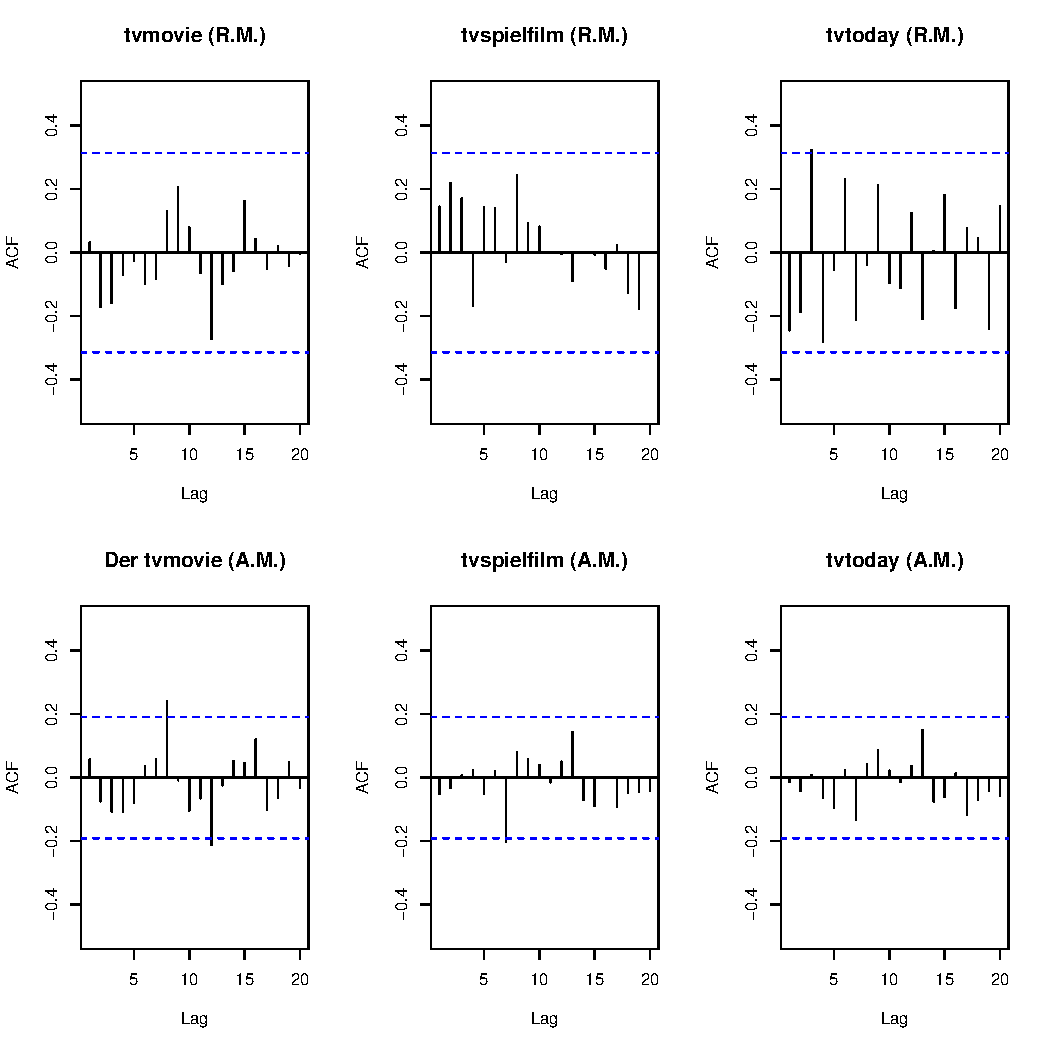
\includegraphics[scale=.6]{resid_acf_tv.eps}
\end{figure}

\begin{figure}[H]
\caption{Residual ACF: women's magazines}
	\centering
	\includegraphics[scale=.6]{resid_acf_frauen.eps}
\end{figure}

\section{Granger Causality}

\begin{table}[!htbp] \centering 
  \caption{Granger Causality test: program guides} 
  \label{tab_granger_tv} 
\begin{tabular}{@{\extracolsep{5pt}} lll} 
\\[-1.8ex]\hline 
\hline \\[-1.8ex] 
 & Test-statisitcs \\ 
\hline \\[-1.8ex] 
 & sales & advertising pages/copy\\
\hline \\[-1.8ex]
TV Movie --\textgreater  TV Spielfilm & $8.4232^{**}$ & $1.6847$\\ 
TV Movie --\textgreater  TV Digital & $6.5797^{**}$ & $.00704$ \\ 
\hline
TV Spielfilm --\textgreater  TV Movie & $.3115$ & $1.0383$ \\ 
TV Spielfilm --\textgreater  TV Digital & $2.6609$ & $4.1236^{**}$ \\ 
\hline
TV Digital --\textgreater  TV Movie & $6.1264^{**}$ & $.58604$\\ 
TV Digital --\textgreater  TV Spielfilm & $3.0848$ & $.36953$\\ 
\hline \\[-1.8ex]
\end{tabular} 
\end{table}

\begin{table}[!htbp] \centering 
  \caption{Granger Causality test: women's magazines} 
  \label{tab_granger_frauen} 
\begin{tabular}{@{\extracolsep{5pt}} lll} 
\\[-1.8ex]\hline 
 & sales & advertising pages/copy\\
\hline \\[-1.8ex] 
 & Test-statisitcs \\ 
\hline \\[-1.8ex] 
Brigitte --\textgreater  Freundin & $.56607$ & $.29108$\\ 
Brigitte --\textgreater  Für Sie & $2.9389^{*}$ & $2.8954^{*}$ \\ 
\hline
Freundin --\textgreater  Brigitte & $.45525$ & $5.7894^{*}$ \\ 
Freundin --\textgreater  Für Sie & $3.3437^{*}$ & $.35349$ \\ 
\hline
Für Sie --\textgreater  Brigitte & $1.4086$ & $1.2124$\\ 
Für Sie --\textgreater  Freundin & $.00694$ & $2.7476^{*}$\\ 
\hline \\[-1.8ex]
\end{tabular} 
\end{table}



\end{appendices}


\end{document}
